% Options for packages loaded elsewhere
\PassOptionsToPackage{unicode}{hyperref}
\PassOptionsToPackage{hyphens}{url}
%
\documentclass[
  ignorenonframetext,
  aspectratio=169]{beamer}
\usepackage{pgfpages}
\setbeamertemplate{caption}[numbered]
\setbeamertemplate{caption label separator}{: }
\setbeamercolor{caption name}{fg=normal text.fg}
\beamertemplatenavigationsymbolsempty
% Prevent slide breaks in the middle of a paragraph
\widowpenalties 1 10000
\raggedbottom
\setbeamertemplate{part page}{
  \centering
  \begin{beamercolorbox}[sep=16pt,center]{part title}
    \usebeamerfont{part title}\insertpart\par
  \end{beamercolorbox}
}
\setbeamertemplate{section page}{
  \centering
  \begin{beamercolorbox}[sep=12pt,center]{part title}
    \usebeamerfont{section title}\insertsection\par
  \end{beamercolorbox}
}
\setbeamertemplate{subsection page}{
  \centering
  \begin{beamercolorbox}[sep=8pt,center]{part title}
    \usebeamerfont{subsection title}\insertsubsection\par
  \end{beamercolorbox}
}
\AtBeginPart{
  \frame{\partpage}
}
\AtBeginSection{
  \ifbibliography
  \else
    \frame{\sectionpage}
  \fi
}
\AtBeginSubsection{
  \frame{\subsectionpage}
}
\usepackage{amsmath,amssymb}
\usepackage{lmodern}
\usepackage{iftex}
\ifPDFTeX
  \usepackage[T1]{fontenc}
  \usepackage[utf8]{inputenc}
  \usepackage{textcomp} % provide euro and other symbols
\else % if luatex or xetex
  \usepackage{unicode-math}
  \defaultfontfeatures{Scale=MatchLowercase}
  \defaultfontfeatures[\rmfamily]{Ligatures=TeX,Scale=1}
\fi
\usetheme[]{Frankfurt}
\usecolortheme{beaver}
% Use upquote if available, for straight quotes in verbatim environments
\IfFileExists{upquote.sty}{\usepackage{upquote}}{}
\IfFileExists{microtype.sty}{% use microtype if available
  \usepackage[]{microtype}
  \UseMicrotypeSet[protrusion]{basicmath} % disable protrusion for tt fonts
}{}
\makeatletter
\@ifundefined{KOMAClassName}{% if non-KOMA class
  \IfFileExists{parskip.sty}{%
    \usepackage{parskip}
  }{% else
    \setlength{\parindent}{0pt}
    \setlength{\parskip}{6pt plus 2pt minus 1pt}}
}{% if KOMA class
  \KOMAoptions{parskip=half}}
\makeatother
\usepackage{xcolor}
\newif\ifbibliography
\setlength{\emergencystretch}{3em} % prevent overfull lines
\providecommand{\tightlist}{%
  \setlength{\itemsep}{0pt}\setlength{\parskip}{0pt}}
\setcounter{secnumdepth}{-\maxdimen} % remove section numbering
% % set background image if you will
% \usebackgroundtemplate%
% {%
%     \includegraphics[width=\paperwidth,height=\paperheight]{02-dna_modification_background_dna_helix.jpg}%
% }

% % set caption font size
% % note that beamer presentation native captions have their own configs
% \usepackage{caption}
% \captionsetup{font=footnotesize}

% this font option is amenable for beamer
\setbeamerfont{caption}{size=\tiny}

% some beamer themes naturally might not support navigation symbols
% \setbeamertemplate{navigation symbols}{} % remove navigation symbols

\setbeamertemplate{footline}[page number] % insert page number in footline

% \setbeamertemplate{navigation symbols}{slide} % insert slide indication in navigation
% \setbeamertemplate{navigation symbols}{frame} % insert frame indication in navigation
% \setbeamertemplate{navigation symbols}{section} % insert section indication in navigation
% \setbeamertemplate{navigation symbols}{subsection} % insert subsection indication in navigation

% \AtBeginSubsection{} % supress subsection display

\newcommand{\bcolumns}{\begin{columns}[T, onlytextwidth]}
\newcommand{\ecolumns}{\end{columns}}

\newcommand{\bdescription}{\begin{description}}
\newcommand{\edescription}{\end{description}}

\newcommand{\bitemize}{\begin{itemize}}
\newcommand{\eitemize}{\end{itemize}}
\AtBeginSubsection{}
\ifLuaTeX
  \usepackage{selnolig}  % disable illegal ligatures
\fi
\usepackage[]{natbib}
\bibliographystyle{plainnat}
\IfFileExists{bookmark.sty}{\usepackage{bookmark}}{\usepackage{hyperref}}
\IfFileExists{xurl.sty}{\usepackage{xurl}}{} % add URL line breaks if available
\urlstyle{same} % disable monospaced font for URLs
\hypersetup{
  pdftitle={Applications of tissue culture for crop improvement},
  pdfauthor={Deependra Dhakal},
  hidelinks,
  pdfcreator={LaTeX via pandoc}}

\title{Applications of tissue culture for crop improvement}
\author{Deependra Dhakal}
\date{}
\institute{Agriculture and Forestry University}

\begin{document}
\frame{\titlepage}

\begin{frame}[allowframebreaks]
  \tableofcontents[hideallsubsections]
\end{frame}
\hypertarget{haploid-and-triploid-production}{%
\section{Haploid and triploid
production}\label{haploid-and-triploid-production}}

\hypertarget{haploid-production}{%
\subsection{Haploid production}\label{haploid-production}}

\begin{frame}{Haploid production}
\begin{itemize}
\tightlist
\item
  In nature, haploids occur at 0.001-0.01\% frequency.
\item
  Spontaneous production of haploids, usually occurs through
  parthenogenesis, but rarely though `ovule androgenesis'.
\item
  Until 1964, artificial production of haploids was attempted through:

  \begin{itemize}
  \tightlist
  \item
    Distant hybridization
  \item
    Delayed pollination
  \item
    Application of irradiated pollen
  \item
    Hormone treatments
  \item
    Temperature shocks
  \end{itemize}
\item
  Guha and Maheshwari, 1964 first reported the development of numerous
  pollen plantlets in anther cultures of \emph{Datura innoxia}.
\end{itemize}
\end{frame}

\hypertarget{distant-hybridization-for-haploid-production}{%
\subsection{Distant hybridization for haploid
production}\label{distant-hybridization-for-haploid-production}}

\begin{frame}{Distant hybridization for haploid production}
\bcolumns
\column{0.6\textwidth}

\begin{center}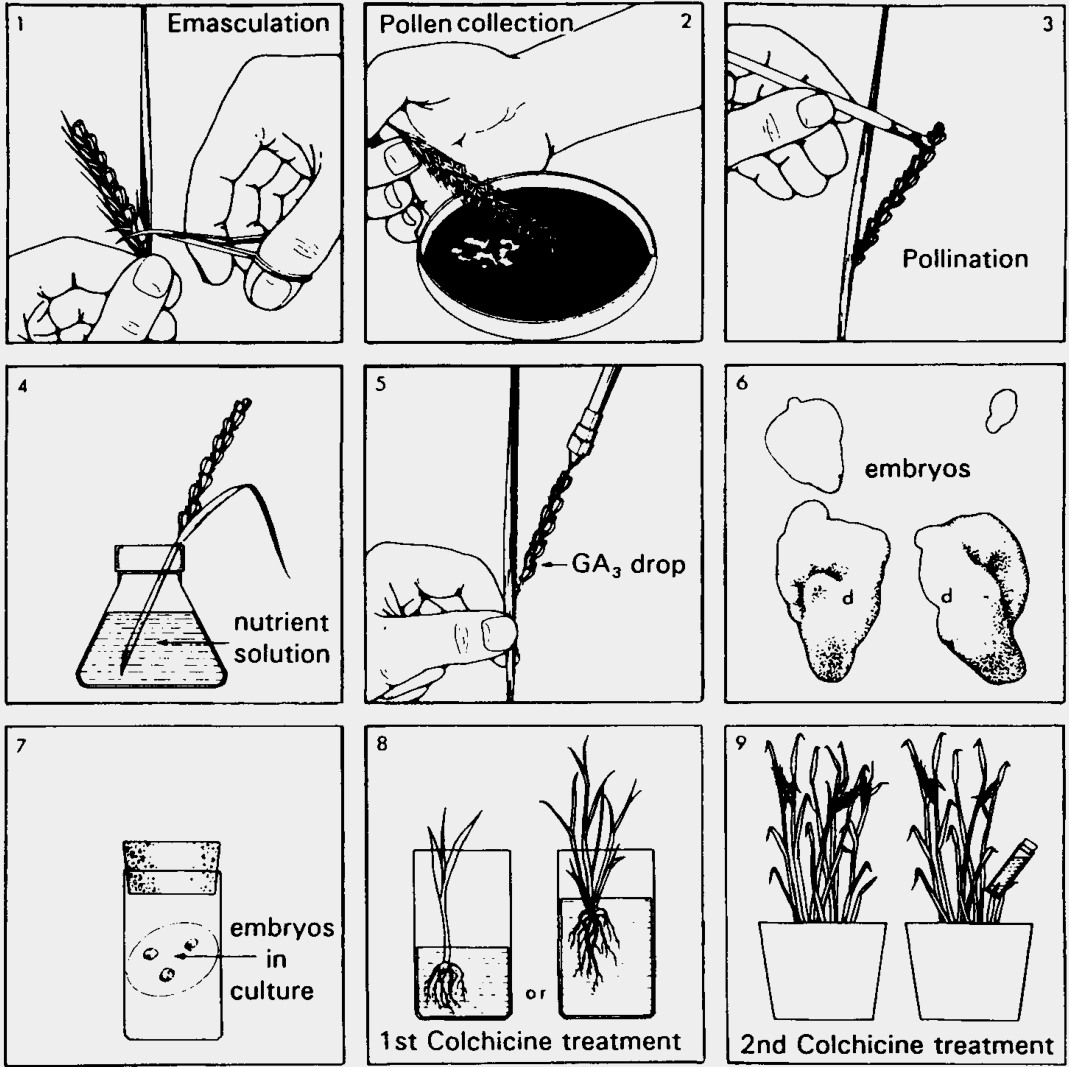
\includegraphics[width=0.82\linewidth]{../images/haploid_production_distant_hybridization} \end{center}

\column{0.4\textwidth}

Interspecific crosses between cultivated barley ( \emph{Hordeum
vulgare}) and the wild species \emph{H. bulbosum} followed by in vitro
culture of rescued immature embryos results in haploid plants as a
result of exclusion of the H. bulbosum chromosomes during embryo
development.

\ecolumns
\end{frame}

\hypertarget{haploid-inducer-lines-in-maize}{%
\subsection{Haploid inducer lines in
Maize}\label{haploid-inducer-lines-in-maize}}

\begin{frame}{Haploid inducer lines in Maize}
\begin{itemize}
\tightlist
\item
  Refer to lecture slide on Polyploidy in plant breeding, Introductory
  Plant Breeding, 4th Semester.
\end{itemize}
\end{frame}

\hypertarget{anther-culture-steps-case-of-cassava}{%
\subsection{Anther culture: Steps (case of
Cassava)}\label{anther-culture-steps-case-of-cassava}}

\begin{frame}{Anther culture: Steps (case of Cassava)}
\begin{enumerate}
\tightlist
\item
  Selection and collection of plant material
\item
  Pre-treatment
\end{enumerate}

\begin{itemize}
\tightlist
\item
  cold pre-treatment for 4 days at 10 degree C
\item
  heat pre-treatment for 24 hours at 37 degree C
\end{itemize}

\begin{enumerate}
\setcounter{enumi}{2}
\tightlist
\item
  Sterilization
\end{enumerate}

\begin{itemize}
\tightlist
\item
  heat (open flame sterilization of flower bud using burner)
\item
  chemical
\end{itemize}

\begin{enumerate}
\setcounter{enumi}{3}
\tightlist
\item
  Separation of anther tissue from flower bud
\item
  Culturing
\end{enumerate}

\begin{itemize}
\tightlist
\item
  androgenesis
\item
  callus proliferation or somatic embryogenesis
\item
  plantlet regeneration
\end{itemize}
\end{frame}

\hypertarget{section}{%
\subsection{}\label{section}}

\begin{frame}{}
\bcolumns
\column{0.4\textwidth}

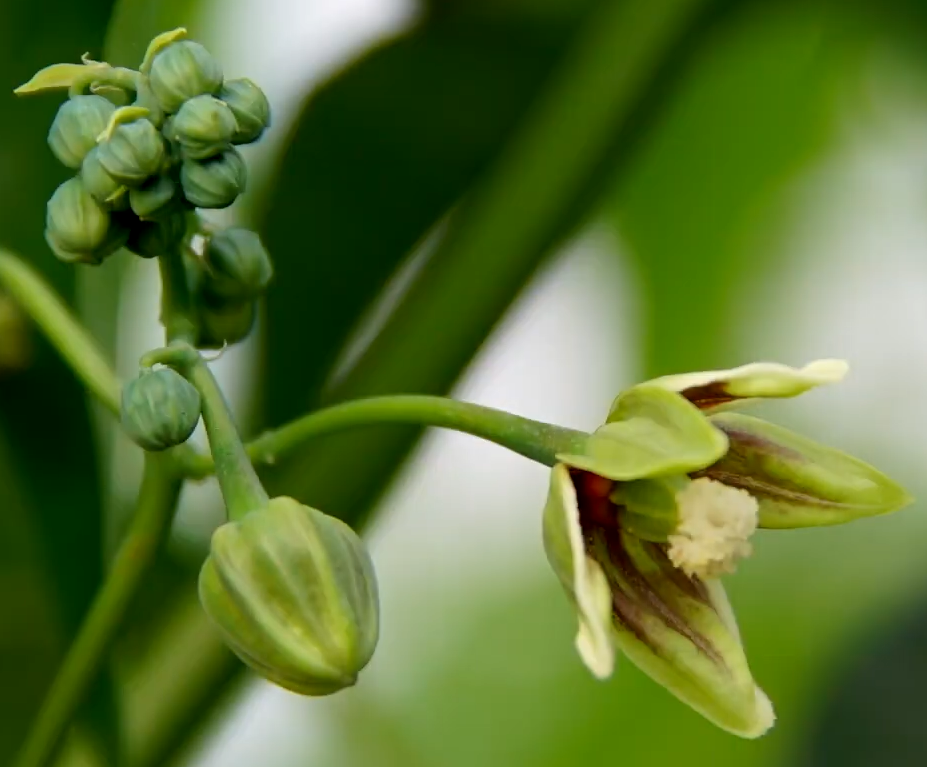
\includegraphics[width=0.8\linewidth]{../images/selection_of_plant_material}

\column{0.3\textwidth}

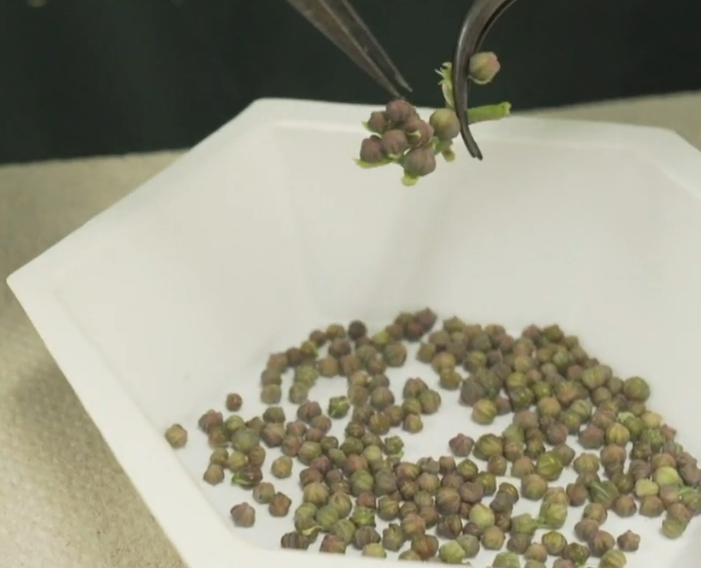
\includegraphics[width=0.95\linewidth]{../images/separation_of_flower}

\column{0.3\textwidth}

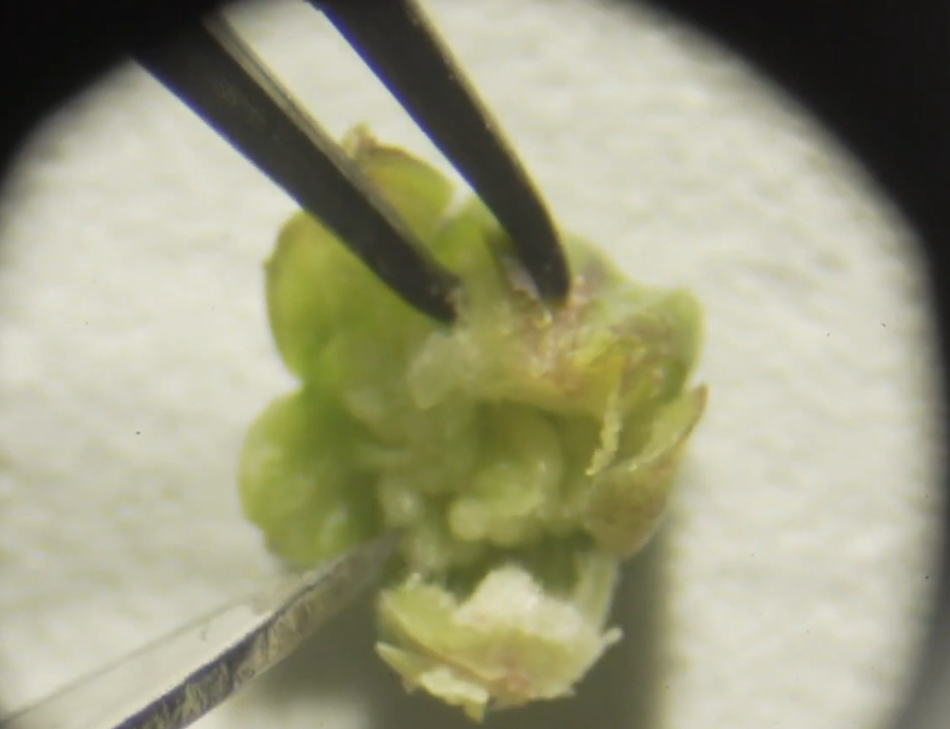
\includegraphics[width=0.95\linewidth]{../images/separation_of_anther}

\ecolumns

\begin{center}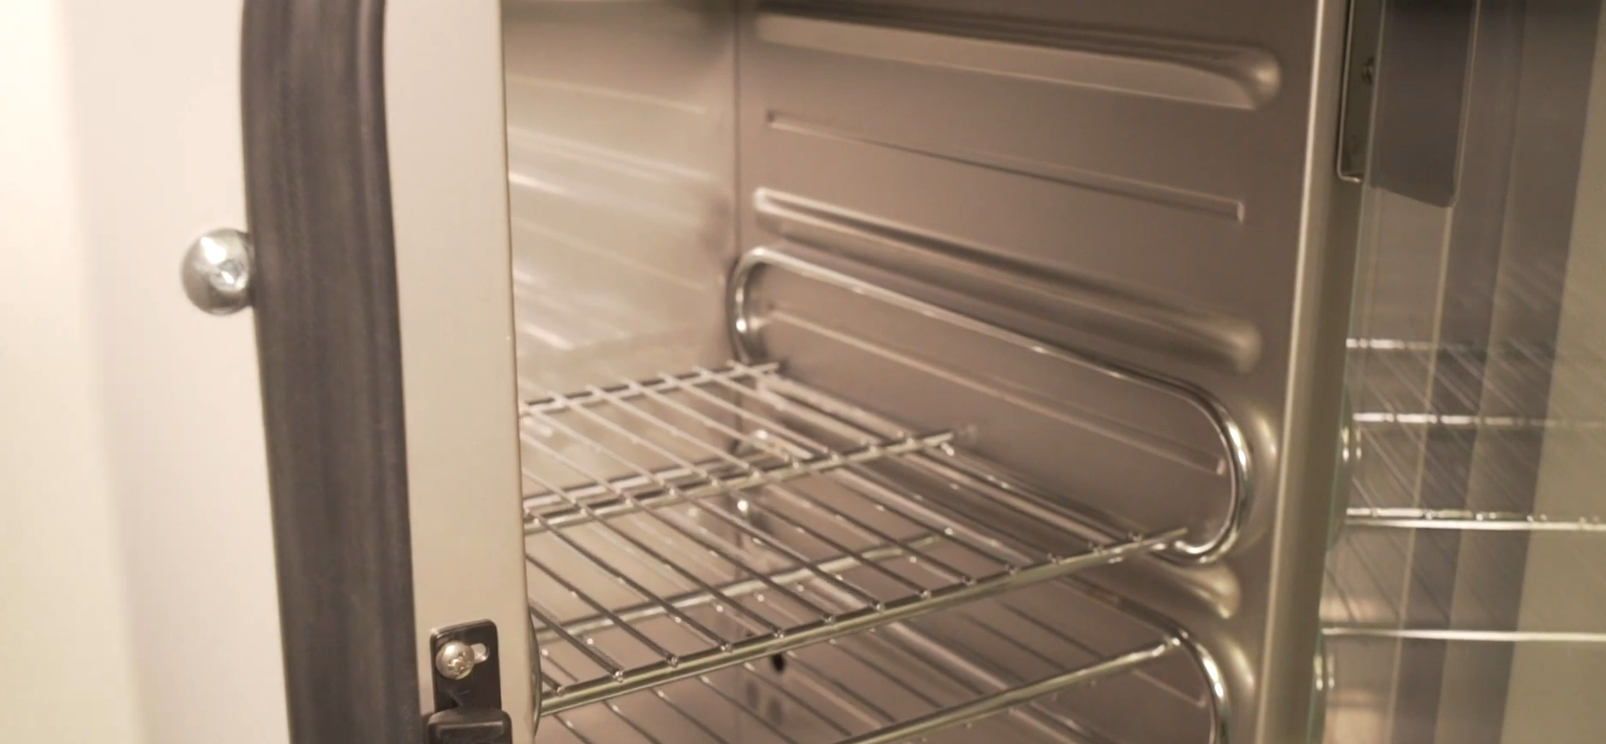
\includegraphics[width=0.52\linewidth]{../images/heat_pretreatment} \end{center}
\end{frame}

\hypertarget{section-1}{%
\subsection{}\label{section-1}}

\begin{frame}{}
\begin{center}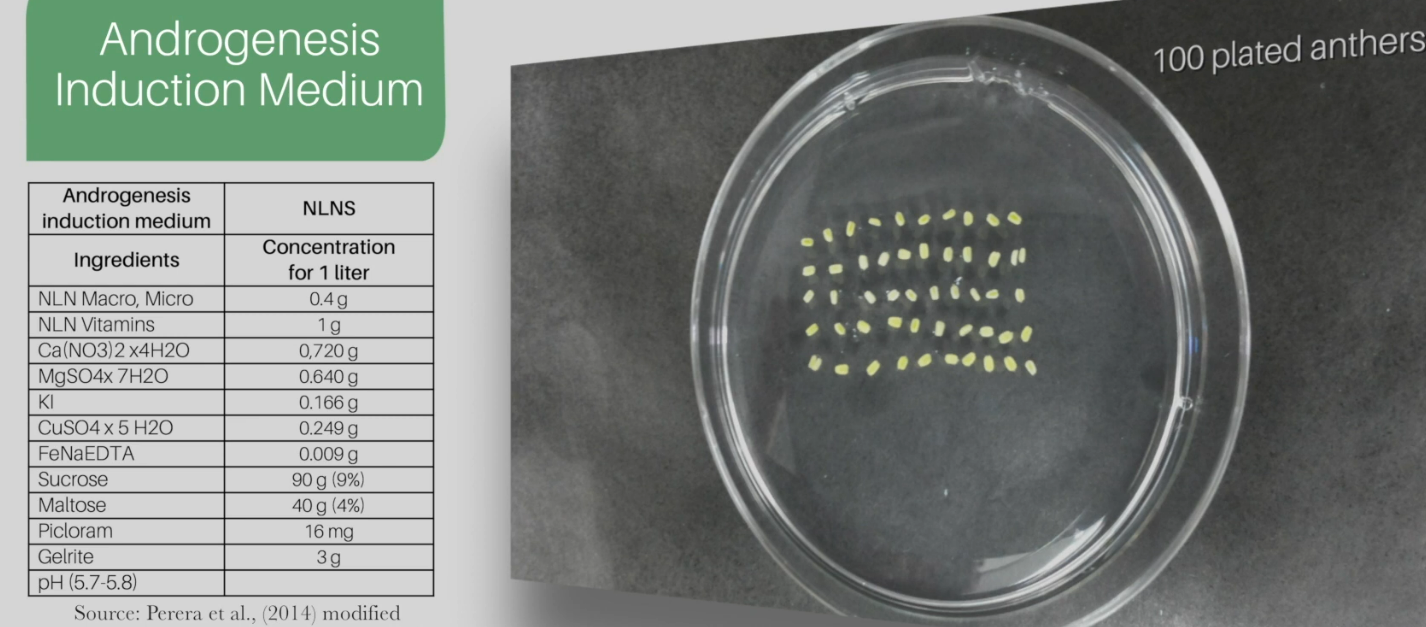
\includegraphics[width=0.48\linewidth]{../images/androgenesis_induction_medium} \end{center}

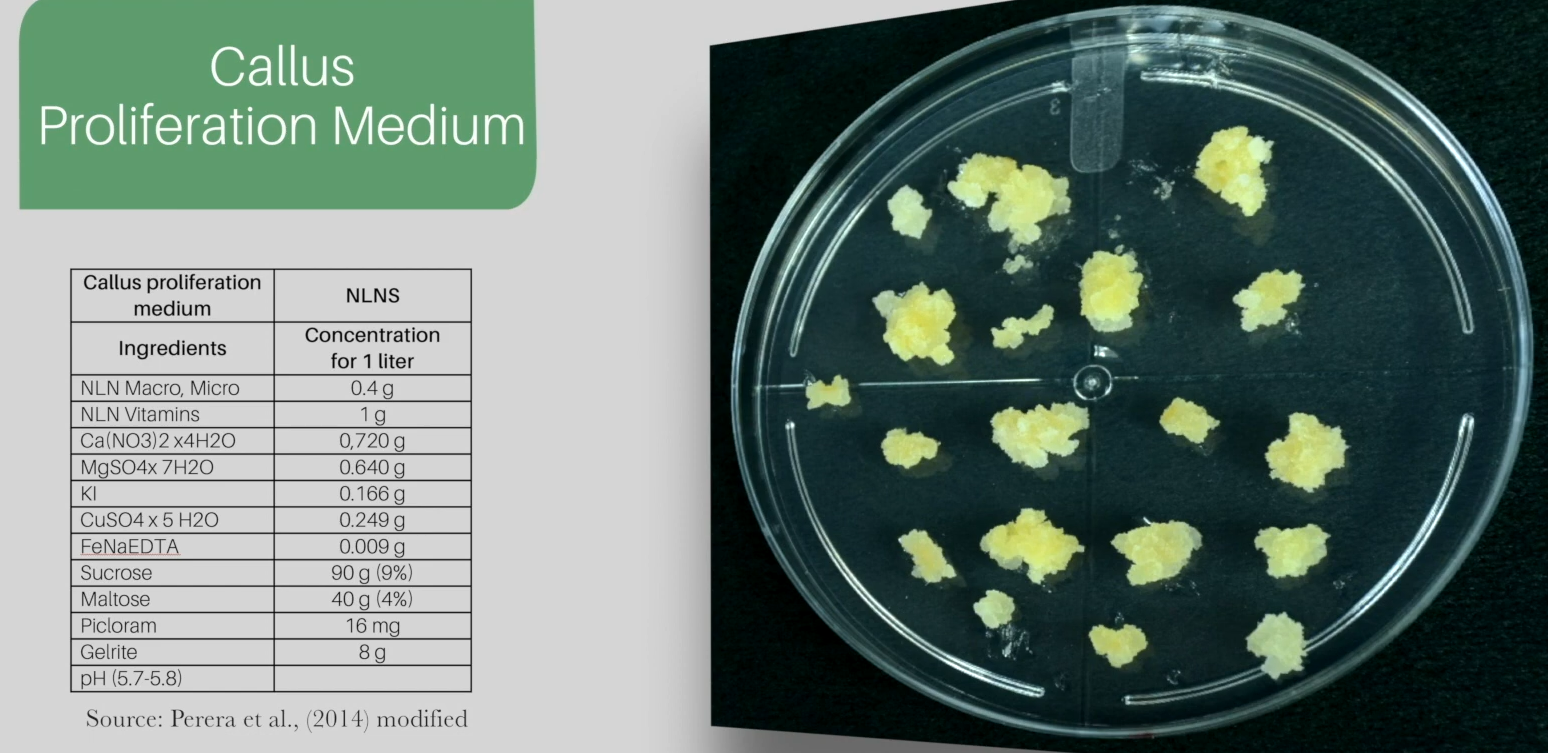
\includegraphics[width=0.48\linewidth]{../images/callus_induction}
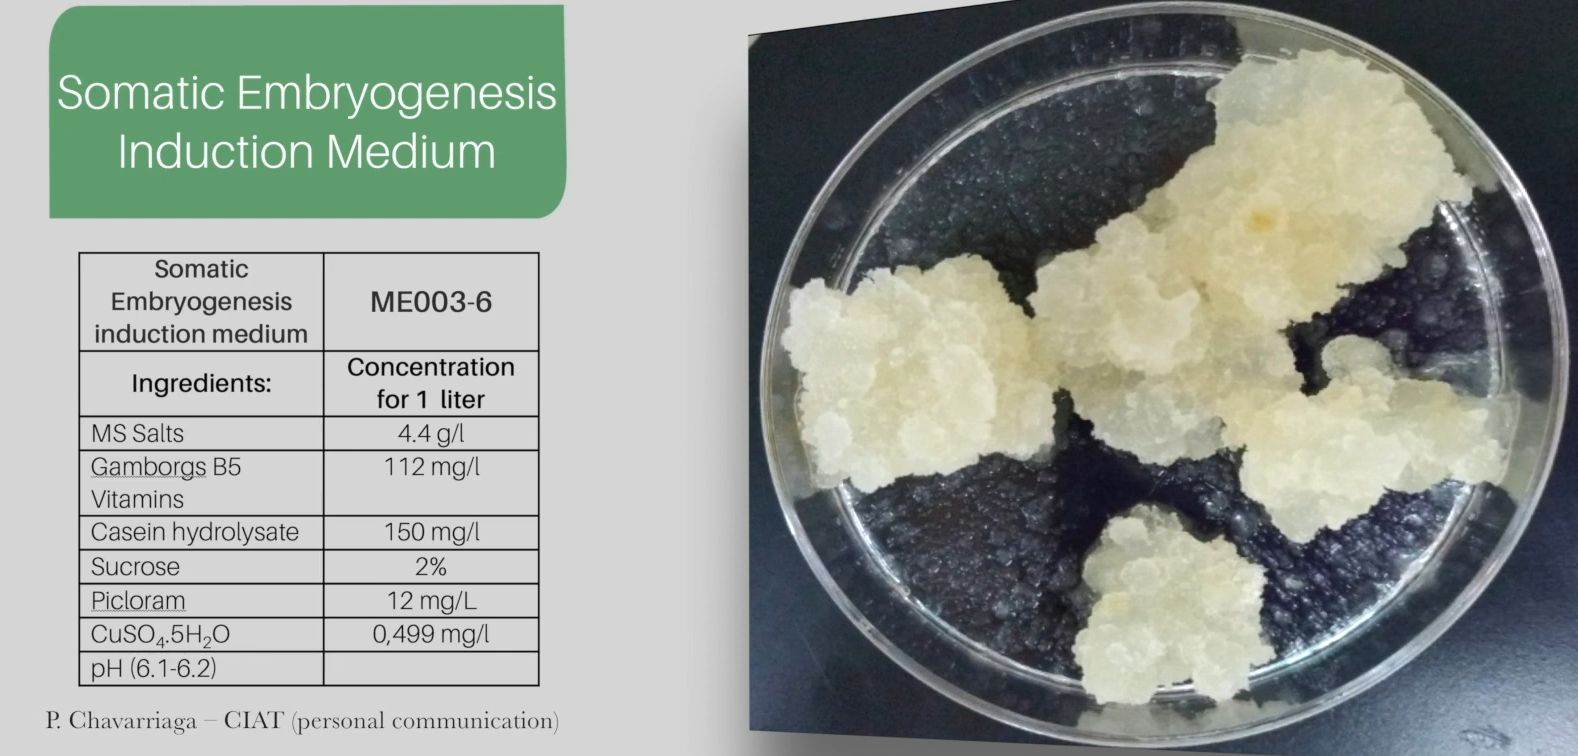
\includegraphics[width=0.48\linewidth]{../images/somatic_embryogenesis_induction}
\end{frame}

\hypertarget{section-2}{%
\subsection{}\label{section-2}}

\begin{frame}{}
\begin{center}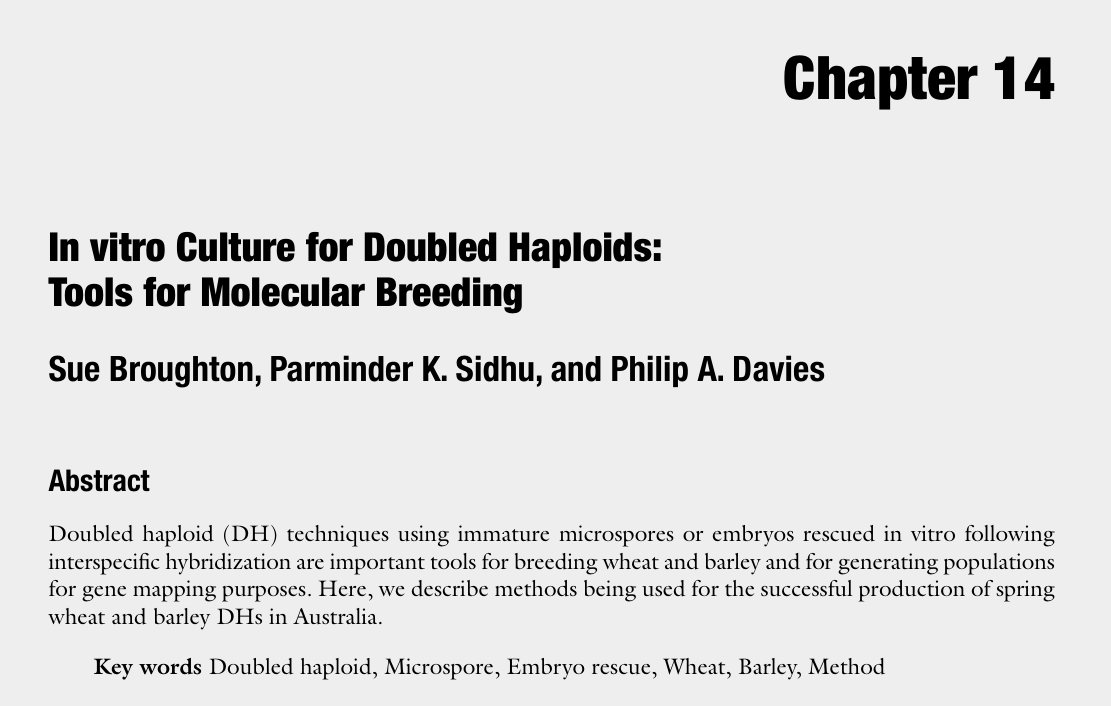
\includegraphics[width=0.6\linewidth]{../images/protocol_double_haploid_production} \end{center}

For protocol based exposition refer to: \citet{broughton2014vitro}
(Book: Crop Breeding Methods and Protocols).
\end{frame}

\hypertarget{triploid-production}{%
\subsection{Triploid production}\label{triploid-production}}

\begin{frame}{Triploid production}
\bcolumns
\column{0.5\textwidth}

\begin{itemize}
\tightlist
\item
  Monoploids: Number of chromosome in a single set of chromosomes
  (denoted by x).
\item
  Dihaploids: Two sets of chromosomes in gametes (gametes of
  tetraploids)
\item
  Polyploidy arises due to:

  \begin{itemize}
  \tightlist
  \item
    Unreduced gametes
  \item
    Polyspermy
  \item
    Chromosome doubling
  \end{itemize}
\item
  Triploids have three copies of monoploid sets
\end{itemize}

\column{0.5\textwidth}

\begin{center}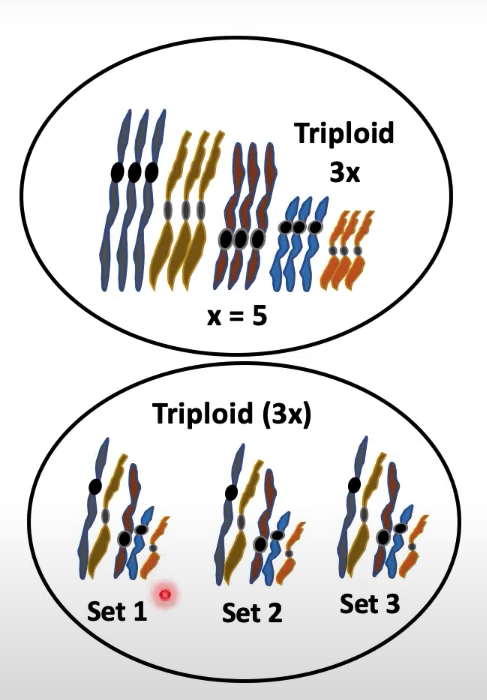
\includegraphics[width=0.58\linewidth]{../images/triploidy} \end{center}

\ecolumns
\end{frame}

\hypertarget{section-3}{%
\subsection{}\label{section-3}}

\begin{frame}{}
\begin{itemize}
\tightlist
\item
  Have several desirable characters such as larger organs -- leaves,
  fruits and flowers.
\item
  Exhibit greater vigor, higher biomass and stress resistance.
\item
  Are sterile and fruits are seedless, i.e., grapes, watermelon, citrus
  fruits etc.
\item
  Natural triploids exist in nature -- \emph{Populus tremula}, \emph{P.
  alba}, \emph{Quercus} spp., \emph{Miscanthus} spp.
\item
  Artificial triploids have been created using wide hybridization
  (example presented in respective section)
\end{itemize}
\end{frame}

\hypertarget{section-4}{%
\subsection{}\label{section-4}}

\begin{frame}{}
\bcolumns
\column{0.5\textwidth}

\textbf{Natural hybridization}

\begin{itemize}
\tightlist
\item
  The success of hybridization depends on

  \begin{itemize}
  \tightlist
  \item
    pollen viability
  \item
    compatibility between parent
  \item
    frequency of unreduced gametes
  \end{itemize}
\end{itemize}

\begin{center}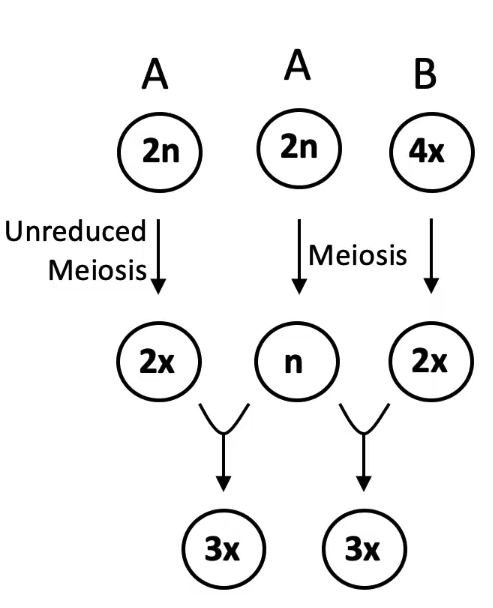
\includegraphics[width=0.6\linewidth]{../images/triploid_production_basis} \end{center}

\column{0.5\textwidth}

\textbf{Artificial/\emph{invitro} fertilization}

\begin{itemize}
\tightlist
\item
  Triploid production could be brought about artificially by

  \begin{itemize}
  \tightlist
  \item
    polyspermy: Fertilization of more than one male gametes with the egg
    cell
  \end{itemize}
\end{itemize}

\begin{center}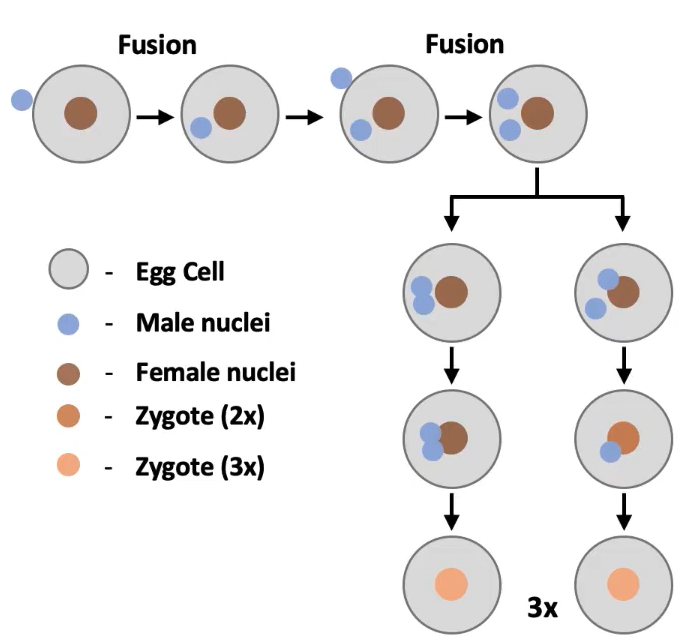
\includegraphics[width=0.6\linewidth]{../images/polyspermy_induced_by_electrofusion} \end{center}

\ecolumns
\end{frame}

\hypertarget{callusing}{%
\subsection{Callusing}\label{callusing}}

\begin{frame}{Callusing}
\begin{itemize}
\tightlist
\item
  Earliest attempt to grow endosperm tissue in culture was made during
  1933.

  \begin{itemize}
  \tightlist
  \item
    Lampe and Mills grew young corn endosperm on a nutrient medium
    enriched with the extract of potato or young corn and obtained
    slight proliferation.
  \end{itemize}
\item
  To ensure good proliferation in cereals, \textbf{young} explant should
  be excised

  \begin{itemize}
  \tightlist
  \item
    9-10 days after pollination in \emph{Lolium perenne}
  \item
    8 DAP in \emph{Triticum aestivum} and \emph{H. vulgare}
  \item
    4-7 DAP in \emph{Oryza sativa}
  \end{itemize}
\item
  In fact, mature cereal endosperm is considered dead.
\item
  However, in tomato endosperm culture is deemed most successful 37-50
  days from fruit-set.
\item
  Initial association of embryo to the endosperm may be necessary for
  inducing proliferation.
\end{itemize}
\end{frame}

\hypertarget{section-5}{%
\subsection{}\label{section-5}}

\begin{frame}{}
\begin{itemize}
\tightlist
\item
  Early culturing media contained supplements such as tomato juice
  (derived from young age fruit has been shown to cause cytokinin-like
  activity), grape juice, green-corn juice, yeast extract (YE) or cow's
  milk.
\item
  Ideally, the media contains 2,4-D, Kinetin and YE or Casein
  hydrolyaste.
\item
  Endosperm callus of maize growth occurs best at sucrose concentration
  of 2-4\%.
\item
  Corn endosperm grows better in dark than in light (opposite in
  \emph{Ricinus})
\item
  Optimum temperature is reported to be around 25 degree C.
\item
  pH of 6.1 is deemed favorable for maize, while several other crops
  respond well at more acidic pH.
\end{itemize}
\end{frame}

\hypertarget{section-6}{%
\subsection{}\label{section-6}}

\begin{frame}{}
\begin{itemize}
\tightlist
\item
  Corn endosperm becomes cellular 3 DAP and divisions continue upto 7-8
  days.
\item
  On a medium fortified with 2,4-D, kinetin, and YE the proliferation of
  mature endosperm begins 10-12 days after inoculation.
\item
  The endosperm tissue is well known for a high degree of
  polyploidization of its cells during in vivo development. It also
  exhibits various kinds of mitotic irregularities such as chromosome
  bridges and laggards.
\end{itemize}
\end{frame}

\hypertarget{applications}{%
\subsection{Applications}\label{applications}}

\begin{frame}{Applications}
\begin{itemize}
\tightlist
\item
  Refer to Chapter 19 (Applications of Triploids in Agriculture), Plant
  Biology and Biotechnology, Volume 2, 2015.
\end{itemize}
\end{frame}

\hypertarget{invitro-pollination-and-fertilization}{%
\section{Invitro pollination and
fertilization}\label{invitro-pollination-and-fertilization}}

\hypertarget{section-7}{%
\subsection{}\label{section-7}}

\begin{frame}{}
\begin{itemize}
\tightlist
\item
  Most common reasons for use of in-vitro techniques in recent years has
  been to crop improvement using gene
  technology\footnote[frame]{For a REALLY long discussion on the topic refer to \cite{bhojwani1986plant} or the more recent \cite{bhojwani2013plant}}.
\item
  Techniques such as invitro fertilization and protoplast fusion enable
  the recombination of genotypes otherwise limited by incompatibility.
\item
  In vitro pollination has been used to overcome crossing barriers in
  interspecific hybridization within the genus \emph{Cucumis}.
\end{itemize}
\end{frame}

\hypertarget{somatic-hybridization-and-cybridization}{%
\section{Somatic hybridization and
cybridization}\label{somatic-hybridization-and-cybridization}}

\hypertarget{section-8}{%
\subsection{}\label{section-8}}

\begin{frame}{}
\begin{itemize}
\item
  Tao et al.~(2004) indicated that cytoplasmic and cytoplasmic-nuclear
  genomes interaction played important roles in yield, low temperature
  tolerance, and some important agronomic traits in japonica rice.
  Further Tao et al.~(2011) detected that cytoplasmic genes had a
  significant effect on grain weight and filled-grain ratio on indica
  rice. In maize , Tang et al.~(2013) reported that plant height and ear
  height are also controlled by cytoplasmic genes.
\item
  Cybrids produced as a result of protoplast fusion between
  \emph{Nicotiana plumbaginifolia} TBR2 mutant and \emph{N. tabacum}
  were resistant to high levels of herbicide atrazine (Menczel et
  al.~1986 ). They also found that these plants were male sterile due to
  the protruding stigma and shorter than normal fi laments of the cybrid
  plants.
\end{itemize}
\end{frame}

\hypertarget{section-9}{%
\subsection{}\label{section-9}}

\begin{frame}{}
\begin{figure}
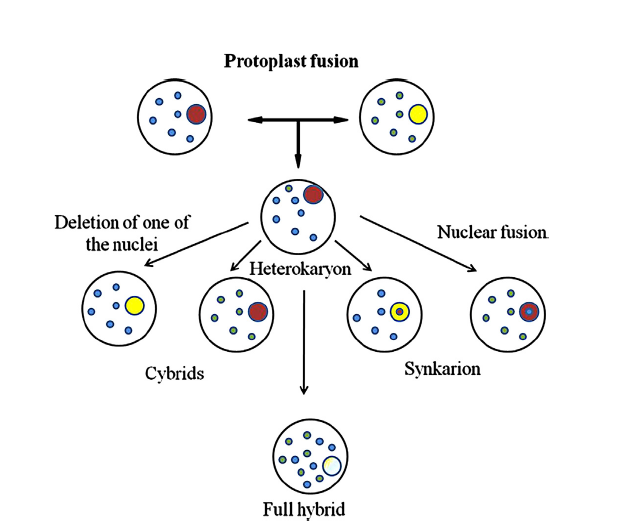
\includegraphics[width=0.6\linewidth]{../images/protoplast_fusion} \caption{Examples of transfer of traits by Protoplast fusion.}\label{fig:traits-transmission-protoplast-fusion}
\end{figure}
\end{frame}

\hypertarget{genetic-transformation-and-wide-hybridization}{%
\section{Genetic transformation and wide
hybridization}\label{genetic-transformation-and-wide-hybridization}}

\hypertarget{section-10}{%
\subsection{}\label{section-10}}

\begin{frame}{}
\begin{itemize}
\tightlist
\item
  Use of invitro techniques in wide hybridization is generally
  associated with the rescue of developing interspecific or intergeneric
  hybrid.
\item
  Embryo rescue involves the excising of embryos and placing them onto
  sterile culture medium.

  \begin{itemize}
  \tightlist
  \item
    Tukey first grew embryo of cherry on an artificial medium in 1933.
  \end{itemize}
\item
  In events of wide hybridization, endosperm develops poorly or does not
  develop at all due to hybridization barriers.

  \begin{itemize}
  \tightlist
  \item
    post-fertilization barriers can be caused by ploidy differences,
    chromosome elimination and seed dormancy.
  \end{itemize}
\end{itemize}
\end{frame}

\hypertarget{section-11}{%
\subsection{}\label{section-11}}

\begin{frame}{}
\begin{itemize}
\tightlist
\item
  Applied in rescuing young embryos of successful interspecific crosses
  of

  \begin{itemize}
  \tightlist
  \item
    \emph{Lycopersicon esculentum} x \emph{L. peruvianum}
  \item
    \emph{Medicago sativa} x \emph{M. rupestris}
  \item
    \emph{Brassica napus x Sinapsis alba}
  \end{itemize}
\item
  Seedless triploid embryos resulting from crosses between diploids and
  tetraploids of the same species.

  \begin{itemize}
  \tightlist
  \item
    Fujiminori (2n = 4x = 76) x Jingxiu (2n = 2x = 38) grape varieties
  \item
    Diploid (2n = 22) x Tetraploid (2n = 44) daylily (
    \emph{Hemerocallis} spp.)
  \end{itemize}
\end{itemize}
\end{frame}

\hypertarget{section-12}{%
\subsection{}\label{section-12}}

\begin{frame}{}
\begin{center}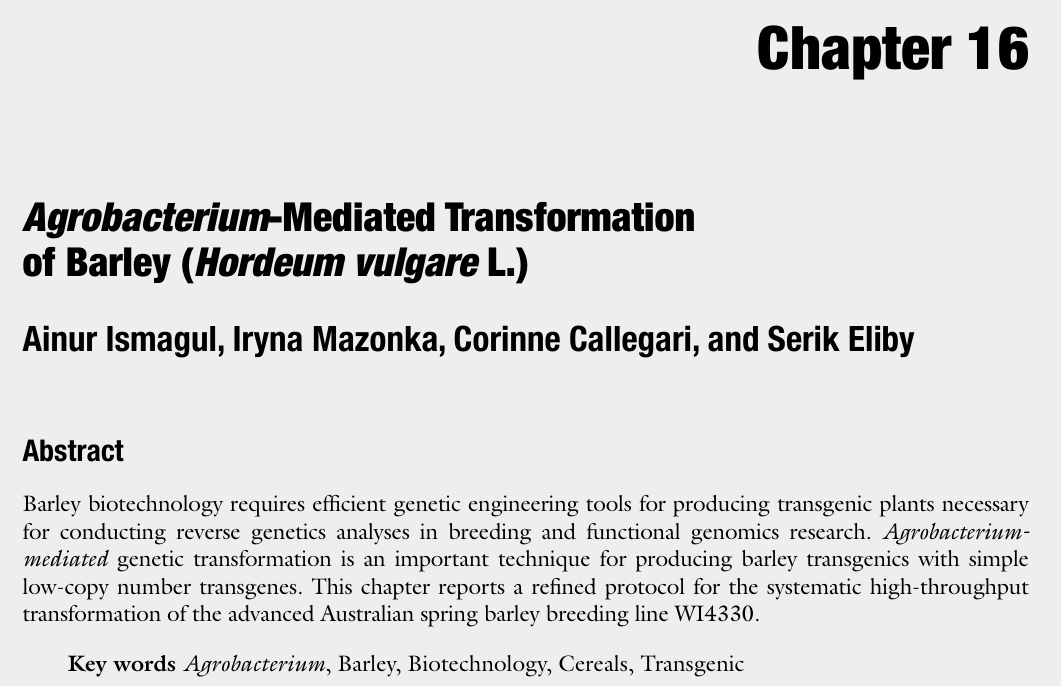
\includegraphics[width=0.55\linewidth]{../images/protocol_agrobacterium_mediated_transformation} \end{center}

For protocol based exposition, refer to:
\citet{ismagul2014agrobacterium}.
\end{frame}

\hypertarget{somaclonalgametoclonal-variants-selection}{%
\section{Somaclonal/gametoclonal variants
selection}\label{somaclonalgametoclonal-variants-selection}}

\hypertarget{section-13}{%
\subsection{}\label{section-13}}

\begin{frame}{}
\begin{itemize}
\tightlist
\item
  Genetic variation, which is essential in plant breeding, is often not
  available under invitro
  conditions\footnote[frame]{For a full 34 page discussion on selecting somaclonal variants, refer to Chapter 9 (Variant selection) of \cite{bhojwani1986plant} or the more recent \cite{bhojwani2013plant}}.
\item
  Jain (1998) suggested that such variation can be induced in-vitro from
  somatic cells or tissues resulting in somaclonal variation leading to
  added genetic variability.
\item
  Characteristics for which somaclonal mutants can be improved during in
  vitro culture includes resistance to disease, herbicides and tolerance
  to environmental or chemical stress, as well as for increased
  production of secondary metabolites.
\item
  Selection is done by employing a stress-causing agent in tissue
  culture containing dividing cells.
\end{itemize}
\end{frame}

\hypertarget{section-14}{%
\subsection{}\label{section-14}}

\begin{frame}{}
\begin{itemize}
\tightlist
\item
  Such variation has been associated with changes in chromosome number
  (ploidy and aneuploidy), chromosome structure, point mutations, and
  DNA methylation -- hence both genetic and epigenetic.
\item
  Molecular markers have been applied successfully to detect somaclonal
  variations of several plant species: \emph{Solanum tuberosum},
  \emph{Gossypium hirsutum} and \emph{Musa} spp.
\end{itemize}
\end{frame}

\renewcommand\refname{Bibliography}
\begin{frame}[allowframebreaks]{Bibliography}
  \bibliographytrue
  \bibliography{../bibliography/bibliographies.bib}
\end{frame}

\end{document}
